%\documentclass[conference]{IEEEtran}
\documentclass{IEEEtran}

% If IEEEtran.cls has not been installed into the LaTeX system files,
% manually specify the path to it like:
% *** MISC UTILITY PACKAGES ***
%
%\usepackage{ifpdf}
% Heiko Oberdiek's ifpdf.sty is very useful if you need conditional
% compilation based on whether the output is pdf or dvi.
% usage:
% \ifpdf
%   % pdf code
% \else
%   % dvi code
% \fi
% The latest version of ifpdf.sty can be obtained from:
% http://www.ctan.org/pkg/ifpdf
% Also, note that IEEEtran.cls V1.7 and later provides a builtin
% \ifCLASSINFOpdf conditional that works the same way.
% When switching from latex to pdflatex and vice-versa, the compiler may
% have to be run twice to clear warning/error messages.

% *** CITATION PACKAGES ***
%
%\usepackage{cite}
% cite.sty was written by Donald Arseneau
% V1.6 and later of IEEEtran pre-defines the format of the cite.sty package
% \cite{} output to follow that of the IEEE. Loading the cite package will
% result in citation numbers being automatically sorted and properly
% "compressed/ranged". e.g., [1], [9], [2], [7], [5], [6] without using
% cite.sty will become [1], [2], [5]--[7], [9] using cite.sty. cite.sty's
% \cite will automatically add leading space, if needed. Use cite.sty's
% noadjust option (cite.sty V3.8 and later) if you want to turn this off
% such as if a citation ever needs to be enclosed in parenthesis.
% cite.sty is already installed on most LaTeX systems. Be sure and use
% version 5.0 (2009-03-20) and later if using hyperref.sty.
% The latest version can be obtained at:
% http://www.ctan.org/pkg/cite
% The documentation is contained in the cite.sty file itself.

\usepackage[T1]{fontenc}
\usepackage[utf8]{inputenc}
\usepackage{xspace}
\usepackage[dvipsnames]{xcolor}
\usepackage{array}
\usepackage{textcomp, parcolumns}
\usepackage{multirow}
\usepackage{tabularx}
\usepackage{enumitem}
\usepackage{colortbl}
\usepackage{listings}
\usepackage{todonotes}




% *** GRAPHICS RELATED PACKAGES ***
%
\ifCLASSINFOpdf
  % \usepackage[pdftex]{graphicx}
  % declare the path(s) where your graphic files are
  % \graphicspath{{../pdf/}{../jpeg/}}
  % and their extensions so you won't have to specify these with
  % every instance of \includegraphics
  % \DeclareGraphicsExtensions{.pdf,.jpeg,.png}
\else
  % or other class option (dvipsone, dvipdf, if not using dvips). graphicx
  % will default to the driver specified in the system graphics.cfg if no
  % driver is specified.
  % \usepackage[dvips]{graphicx}
  % declare the path(s) where your graphic files are
  % \graphicspath{{../eps/}}
  % and their extensions so you won't have to specify these with
  % every instance of \includegraphics
  % \DeclareGraphicsExtensions{.eps}
\fi
% graphicx was written by David Carlisle and Sebastian Rahtz. It is
% required if you want graphics, photos, etc. graphicx.sty is already
% installed on most LaTeX systems. The latest version and documentation
% can be obtained at: 
% http://www.ctan.org/pkg/graphicx
% Another good source of documentation is "Using Imported Graphics in
% LaTeX2e" by Keith Reckdahl which can be found at:
% http://www.ctan.org/pkg/epslatex
%
% latex, and pdflatex in dvi mode, support graphics in encapsulated
% postscript (.eps) format. pdflatex in pdf mode supports graphics
% in .pdf, .jpeg, .png and .mps (metapost) formats. Users should ensure
% that all non-photo figures use a vector format (.eps, .pdf, .mps) and
% not a bitmapped formats (.jpeg, .png). The IEEE frowns on bitmapped formats
% which can result in "jaggedy"/blurry rendering of lines and letters as
% well as large increases in file sizes.
%
% You can find documentation about the pdfTeX application at:
% http://www.tug.org/applications/pdftex





% *** MATH PACKAGES ***
%\usepackage{amsmath}

% *** SPECIALIZED LIST PACKAGES ***
%\usepackage{algorithmic}

% *** ALIGNMENT PACKAGES ***
%\usepackage{array}

% *** SUBFIGURE PACKAGES ***
%\ifCLASSOPTIONcompsoc
%  \usepackage[caption=false,font=normalsize,labelfont=sf,textfont=sf]{subfig}
%\else
%  \usepackage[caption=false,font=footnotesize]{subfig}
%\fi

% *** FLOAT PACKAGES ***
%\usepackage{fixltx2e}
% fixltx2e, the successor to the earlier fix2col.sty, was written by
% Frank Mittelbach and David Carlisle. This package corrects a few problems
% in the LaTeX2e kernel, the most notable of which is that in current
% LaTeX2e releases, the ordering of single and double column floats is not
% guaranteed to be preserved. Thus, an unpatched LaTeX2e can allow a
% single column figure to be placed prior to an earlier double column
% figure.
% Be aware that LaTeX2e kernels dated 2015 and later have fixltx2e.sty's
% corrections already built into the system in which case a warning will
% be issued if an attempt is made to load fixltx2e.sty as it is no longer
% needed.
% The latest version and documentation can be found at:
% http://www.ctan.org/pkg/fixltx2e


%\usepackage{stfloats}
% stfloats.sty was written by Sigitas Tolusis. This package gives LaTeX2e
% the ability to do double column floats at the bottom of the page as well
% as the top. (e.g., "\begin{figure*}[!b]" is not normally possible in
% LaTeX2e). It also provides a command:
%\fnbelowfloat
% to enable the placement of footnotes below bottom floats (the standard
% LaTeX2e kernel puts them above bottom floats). This is an invasive package
% which rewrites many portions of the LaTeX2e float routines. It may not work
% with other packages that modify the LaTeX2e float routines. The latest
% version and documentation can be obtained at:
% http://www.ctan.org/pkg/stfloats
% Do not use the stfloats baselinefloat ability as the IEEE does not allow
% \baselineskip to stretch. Authors submitting work to the IEEE should note
% that the IEEE rarely uses double column equations and that authors should try
% to avoid such use. Do not be tempted to use the cuted.sty or midfloat.sty
% packages (also by Sigitas Tolusis) as the IEEE does not format its papers in
% such ways.
% Do not attempt to use stfloats with fixltx2e as they are incompatible.
% Instead, use Morten Hogholm'a dblfloatfix which combines the features
% of both fixltx2e and stfloats:
%
% \usepackage{dblfloatfix}
% The latest version can be found at:
% http://www.ctan.org/pkg/dblfloatfix




% *** PDF, URL AND HYPERLINK PACKAGES ***
%
%\usepackage{url}
% url.sty was written by Donald Arseneau. It provides better support for
% handling and breaking URLs. url.sty is already installed on most LaTeX
% systems. The latest version and documentation can be obtained at:
% http://www.ctan.org/pkg/url
% Basically, \url{my_url_here}.




% *** Do not adjust lengths that control margins, column widths, etc. ***
% *** Do not use packages that alter fonts (such as pslatex).         ***
% There should be no need to do such things with IEEEtran.cls V1.6 and later.
% (Unless specifically asked to do so by the journal or conference you plan
% to submit to, of course. )


% correct bad hyphenation here
\hyphenation{op-tical net-works semi-conduc-tor}

%STRIDE added as a command, As we will use it many times in future.
\newcommand{\stride}{\emph{STRIDE}}


\begin{document}
%Single level title
%\title{Security analysis of Linux package managers}
%With multilevel title
\title{Security analysis of Linux package manager \\ \vspace{1 mm} {\Large Analyzing and threat modeling of different package managers}}


% author names and affiliations
% use a multiple column layout for up to three different
% affiliations
%\author{\IEEEauthorblockN{Saad Quassil Allak}
%\IEEEauthorblockA{Fachbereich Informatik\\
%	Technische Universit{\"a}t Darmstadt\\
%	Hochschulstra{\ss}e 10 , 64289 Darmstadt\\
%	Email: saadouassil.allak@stud.tu-darmstadt.de}
%\and
%\IEEEauthorblockN{Pranay Sarkar}
%\IEEEauthorblockA{Fachbereich Informatik\\
%	Technische Universit{\"a}t Darmstadt\\
%	Hochschulstra{\ss}e 10 , 64289 Darmstadt\\
%	Email: pranay.sarkar@stud.tu-darmstadt.de}
%}

% Alternate frmat - looks better

\author{\IEEEauthorblockN{Saad Quassil Allak\IEEEauthorrefmark{1},
and
Pranay Sarkar\IEEEauthorrefmark{2}} \\
\IEEEauthorblockA{Fachbereich Informatik\\
	Technische Universit{\"a}t Darmstadt\\
	Hochschulstra{\ss}e 10 , 64289 Darmstadt\\
	\IEEEauthorrefmark{1}
	Email: saadouassil.allak@stud.tu-darmstadt.de \\
	Matriculation Number: --} \\
\IEEEauthorblockA{\IEEEauthorrefmark{2}
	Email: pranay.sarkar@stud.tu-darmstadt.de \\
	Marticulation Number: 2337328
}}



% make the title area
\maketitle

% As a general rule, do not put math, special symbols or citations
% in the abstract
\begin{abstract}
Package managers deals with the task of determining which packages are to be installed on a host and then downloading and installing all those packages along with all of their dependencies. There are different kinds of package managers available and all of them applies different security mechanism providing varying level of usability and resilience to different kind of attacks. Despite having existing security mechanism all of those package managers care vulnerable to man-in-the-middle (MIM) attack and malicious mirror. Security of package managers also depends on security practices of specific Linux distributions. When te distributions use third party mirrors as official mirrors, vulnerabilities can be easily exploited. It is also seen that when some security mechanisms control the location from where client gets the metadata and packages, actually decreases the system security. We explore the case of attacker having a compromised mirror and how it can compromise or crush thousands of clients, and we analyze the threat model using \stride .
\end{abstract}

%General terms
{\bf General Terms:} Security

% Keywords
{\bf Keywords:} Package manager, Package Management, Mirrors, Attack, Reply Attack, Man-in-the-middle (MIM), Threat Modelling, SDL, STRIDE


\IEEEpeerreviewmaketitle

\section{Introduction}
\label{sec:introduction}
\IEEEPARstart{P}{ackage} managers are the most popular way for software distribution for all modern operating systems. \emph{Package} is a software bundled into archives. Package managers provide centralized and privileged mechanism for software management in a system. As package managers needs superuser (i.e. $root$) access to install softwares, security of the installed packages are very important to secure the whole system.

This paper looks into some of the most popular package managers in Linux: APT [1], APT-RPM [2], YaST [4], YUM [5]. These package managers use one of the following four security models: 
\begin{itemize}
	\item No security,
	\item Cryptographic signatures embedded within the packages,
	\item Signatures on the detached package metadata, 
	\item Signatures on the root metadata.
\end{itemize} 
It can be seen that there is an ordering in the amount of security provided by different security models. Having no signatures allows the attacker to do most attacks, followed by having only package signatures, having signatures on detached package metadata and having signatures on root metadata. But there are some usability problems with some mechanisms. For example, signatures on root metadata do not provide a convenient way to verify \emph{stand-alone package}, which might be obtained from a source other than the main repository. So in those cases users can install those packages even without using security checks. But those package managers which use signatures on detached package metadata or signatures on packages, can easily verify \emph{stand-alone packages}.

It is recommended to combine two of these techniques together and create one layered approach for providing better security. (e.g. signatures on root metadata and signatures on packages or package metadata). This kind of layered approach was first added to Stork [6] package manager and now it is popular throughout the world.

Vulnerabilities are not always exploitable in real world. By looking into security structure of popular distributions, we found that it is necessary for an attacker to control an official mirror for package distribution system (e.g. Debian, Ubuntu, Fedora, OpenSUSE, CentOS). Otherwise attacker can not even launch attack on clients. Many distributions use mechanism for distributing requests to multiple mirrors or provide certain part of information from trusted source. But it can be seen from our analysis that it actually decrease the security of the system and thereby making the attacks easier. 
% Description of rest of the paper
\newline Remaining part of the paper is organized as follows. In section 2, system arcitecture of package managers are described. Section 3 consist threat modeling, which includes types of attacks and different approaches to threat modeling. Section 4 describes our approach to threat modelling and application of \stride. Result of our threat modelling and comparison of effects are described in Section 5.
\section{System Architecture of Package Managers}
\label{sec:sys-architecture}
System architecture description of package managers.

\section{Threat Modelling}
\label{sec:threat-modelling}
Threat model involves attacker who can respond to legitimate requests made by a package manager. One example could be man-in-the-middle \emph{(MIM)}, where the attacker have tricked the client into contacting the wrong compromised server. It can also be a case where user have gained control over an official package distribution mirror. Threat model is described as follows:

\begin{itemize}
	\item Attacker can send arbitary files to the user/client
	\item Attacker does know beforehand what the client is going to request
	\item Attacker does not have any trusted key to sign packages, package metadata or root metadata. As the mirrors does not get the private key to sign files as they only copy the already signed files from the main repository.
	\item Attacker have access to outdated packages, package metadata and root metadata. As there are many outdated repositories openly available to all.
	\item Attacker knows the vulnerabilities in some outdated packages and can exploit those vulnerabilities. Attacker can gain knowledge of this by going through the change-logs of updates or just by using some exploit toolkit.
	\item Attacker have no knowledge of vulnerability of latest version of package (i.e. zero-day vulnerabilities).
	\item If signatures are supported by package managers, it is used. But if there are any client or distribution who choose not to use signature supported by package managers, they are more vulnerable to attack.
	\item If supported and if current root metadata does not contain vulnerable versions of the package, expiration time for root metadata are used. As this root metadata is small file, it is feasible to sign it frequently. 
\end{itemize}

\subsection{Types of Attacks}
\label{subsec:attack-types}
Based on the above mentioned threat model, there can be many type of attacks which can be done on a client. All of the attacks can be used either to crash or control client's computer. Although the impact can vary for different types of attack, all of the attacks can be effective on some package managers:
\begin{itemize}
	\item \emph{Arbitrary Package:} Attacker provides a different package created by them in place of the real package to the user who wants to install it.
	
	\item \emph{Reply Attack:} Attacker replays older versions of request package which are correctly signed but contains security vulnerability. Attacker can then exploit the already existing vulnerability. It should be noted that package managers will never downgrade any existing package. So reply attack will not work while updating existing package. But it will work only when installing new package.
	
	\item \emph{Freeze Attack:} Attacker freezes the information that the client sees to the current point of time, so that client can not see any more updates. It works in the similar way how freeze attack, where wrong metadata is provided to clients. The main goal of this attack is to compromise clients which already have installed vulnerable packages. This attack can also be used to prevent updates in addition of installing a out of date package.
	
	\item \emph{Endless Data:} Attacker returns endless stream of data in response to any download request from an already compromised mirror. This might result in package manager filling up the disk or memory on the client machine and thereby crushing it.
	
	\item \emph{Extraneous Dependencies:} Attacker overwrites package metadata so that addition packages have to be installed as a dependency along with the original package that the user want to install. If the package that is installed as a dependency have security vulnerability, it allows the attacker to compromise the system of the user. For example, if metadata of a package $foo$ states that it depends on another package $bar$, it will cause the package $bar$ to be installed even if it is not desired or needed. And, if this $bar$ is vulnerable, the whole system can be compromised.
\end{itemize}

\subsection{Approaches to Threat Modelling}
\label{subsec:approach-threat-modelling}
Threat modelling can be approached in three different ways.
\begin{itemize}
	\item \emph{Attacker-Centric:} It mainly deals with the techniques of determining thee opponents (i.e. attackers). It also determines and categorizes the different ways by which attacks can act.
	
	\item \emph{Software-Centric:} This kind of threat modeling tries to determine the possible ways by which the sofware and therefore the user is vulnerable to attacks. It also categorizes the types of attacks that can be performed on the specific software.
	
	\item \emph{Asset-centric:} This kind of modeling determines what exactly to protect in the system. It can be different types of data. It also classifies the different levels of assets which can have different levels of effect on the system, if compromised to attackers.
\end{itemize}

\section{Approach \& Tools used}
\label{sec:tools-used}
We have mainly concentrated on threat modeling in software development. For that we have used \emph{Microsoft SDL Threat Modeling}. It works in the following steps: 
\begin{enumerate}
	\item \emph{Describe System:} It describes the individual components of the whole system, as well as the relationship and interaction between the components. 
	\item \emph{Create Checklist:} After that a checklist if created. In this checklist all kind of possible attack scenarios are described for the overall system.
	\item \emph{Access impact and find countermeasures for each item:} The last step is to check the already created checklist, and measuring the possible impact of all possible attacks. Possible countermeasures are also be listed during executing this step.
\end{enumerate}

We have described and analyzed all steps in threat model using \stride. We give them as an input to \stride and \stride analyzes the model, ad generates the report automatically. We can also give the system model as n input to \stride. 

As shown in \emph{Figure 2}
\begin{figure}[ht]
	\centering
	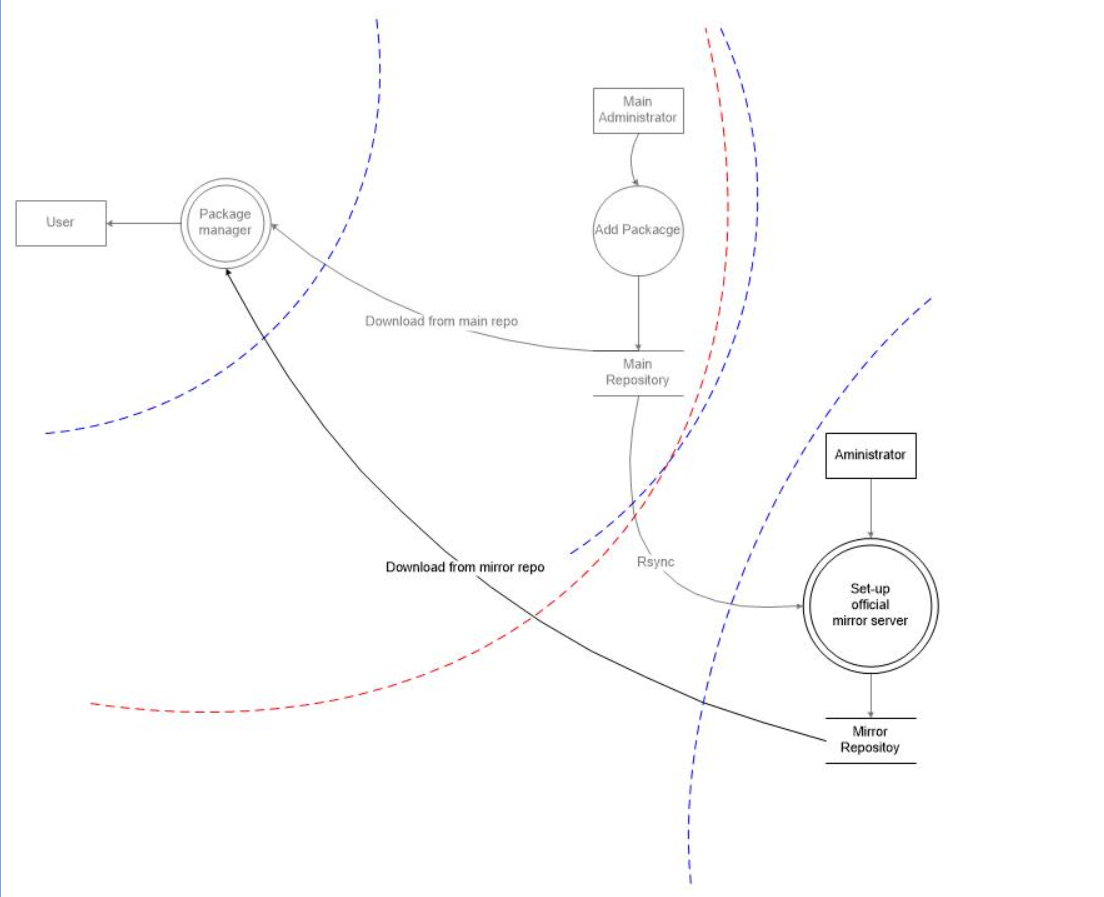
\includegraphics[width=1.0\linewidth]{figures/model}
	\caption[Partial model for motivation example Android app version]{\label{f:stridemodel}System threat model diagram}
\end{figure}

\begin{figure}[ht]
	\centering
	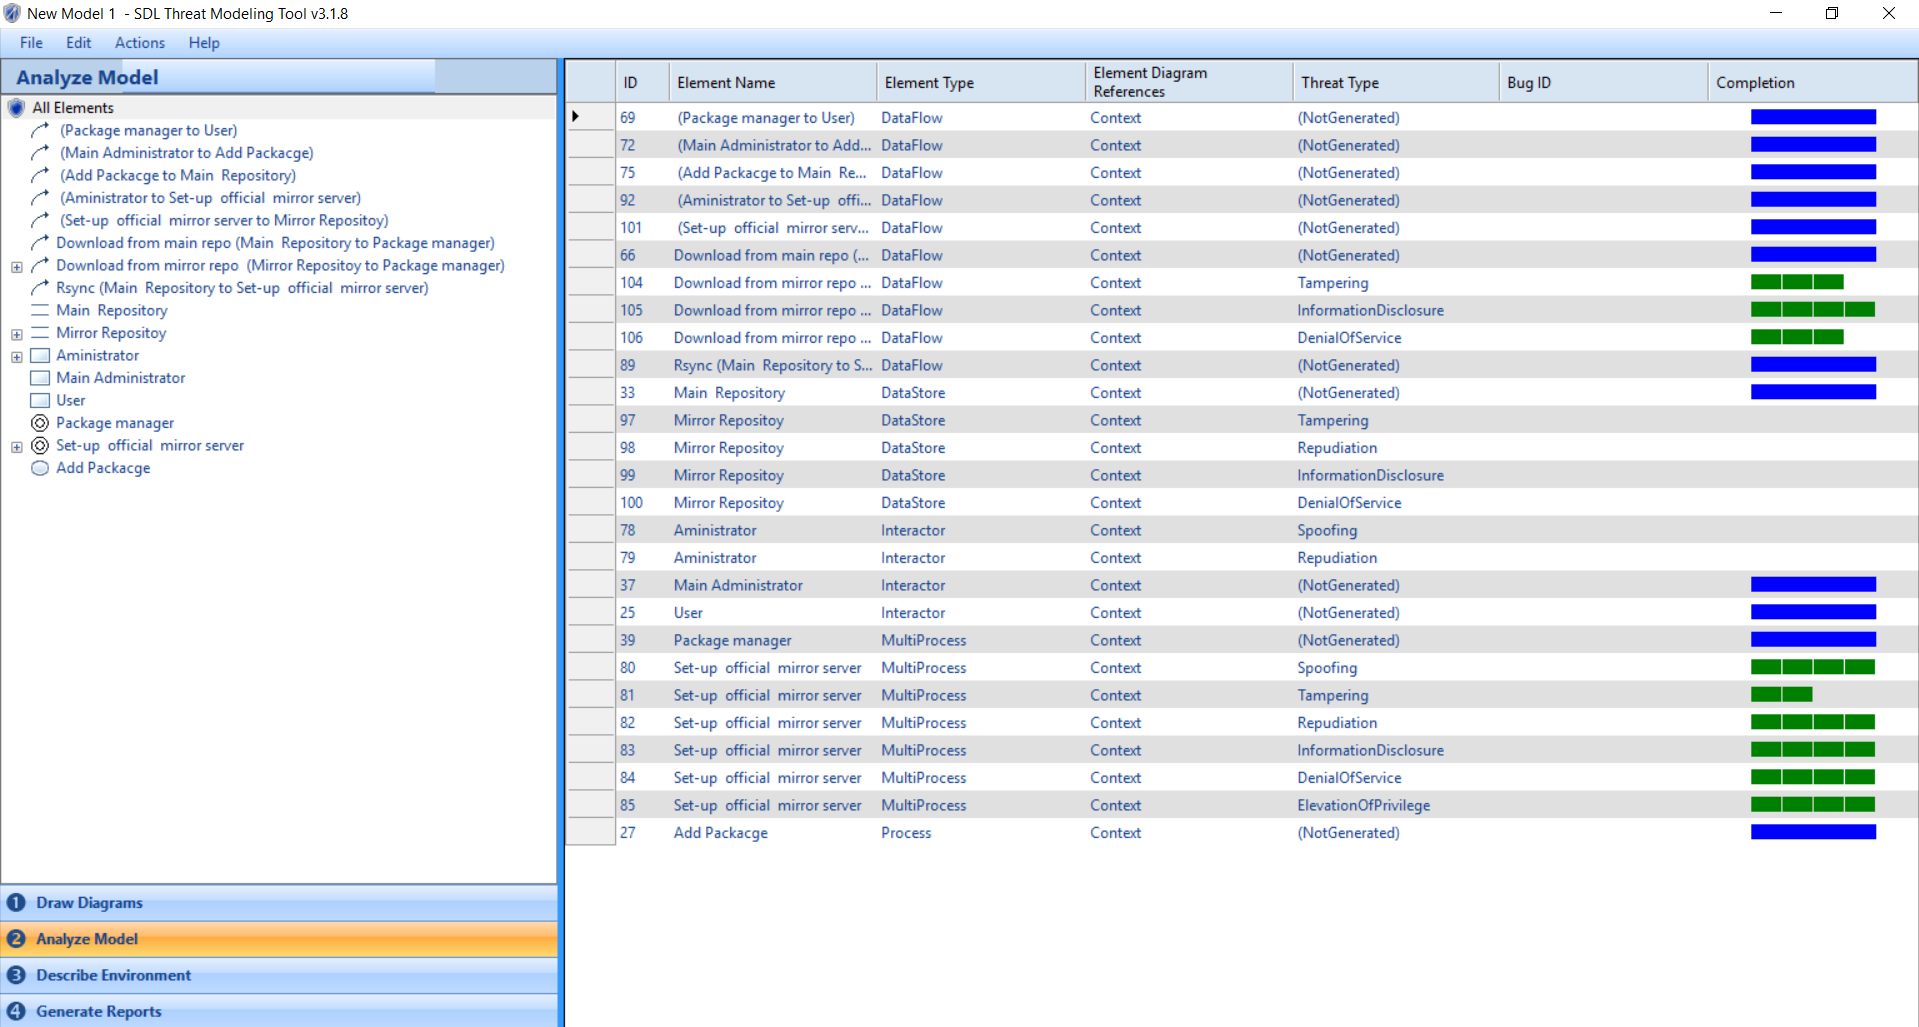
\includegraphics[width=1.0\linewidth]{figures/analyze-model}
	\caption[Partial model for motivation example Android app version]{\label{f:stridemodel}Result of analyzing model in \stride}
\end{figure}

 
%
%\begin{figure}[!t]
%\centering
%\includegraphics[width=2.5in]{myfigure}
% where an .eps filename suffix will be assumed under latex, 
% and a .pdf suffix will be assumed for pdflatex; or what has been declared
% via \DeclareGraphicsExtensions.
%\caption{Simulation results for the network.}
%\label{fig_sim}
%\end{figure}

% Note that the IEEE typically puts floats only at the top, even when this
% results in a large percentage of a column being occupied by floats.


% An example of a double column floating figure using two subfigures.
% (The subfig.sty package must be loaded for this to work.)
% The subfigure \label commands are set within each subfloat command,
% and the \label for the overall figure must come after \caption.
% \hfil is used as a separator to get equal spacing.
% Watch out that the combined width of all the subfigures on a 
% line do not exceed the text width or a line break will occur.
%
%\begin{figure*}[!t]
%\centering
%\subfloat[Case I]{\includegraphics[width=2.5in]{box}%
%\label{fig_first_case}}
%\hfil
%\subfloat[Case II]{\includegraphics[width=2.5in]{box}%
%\label{fig_second_case}}
%\caption{Simulation results for the network.}
%\label{fig_sim}
%\end{figure*}
%
% Note that often IEEE papers with subfigures do not employ subfigure
% captions (using the optional argument to \subfloat[]), but instead will
% reference/describe all of them (a), (b), etc., within the main caption.
% Be aware that for subfig.sty to generate the (a), (b), etc., subfigure
% labels, the optional argument to \subfloat must be present. If a
% subcaption is not desired, just leave its contents blank,
% e.g., \subfloat[].


% An example of a floating table. Note that, for IEEE style tables, the
% \caption command should come BEFORE the table and, given that table
% captions serve much like titles, are usually capitalized except for words
% such as a, an, and, as, at, but, by, for, in, nor, of, on, or, the, to
% and up, which are usually not capitalized unless they are the first or
% last word of the caption. Table text will default to \footnotesize as
% the IEEE normally uses this smaller font for tables.
% The \label must come after \caption as always.
%
%\begin{table}[!t]
%% increase table row spacing, adjust to taste
%\renewcommand{\arraystretch}{1.3}
% if using array.sty, it might be a good idea to tweak the value of
% \extrarowheight as needed to properly center the text within the cells
%\caption{An Example of a Table}
%\label{table_example}
%\centering
%% Some packages, such as MDW tools, offer better commands for making tables
%% than the plain LaTeX2e tabular which is used here.
%\begin{tabular}{|c||c|}
%\hline
%One & Two\\
%\hline
%Three & Four\\
%\hline
%\end{tabular}
%\end{table}


% Note that the IEEE does not put floats in the very first column
% - or typically anywhere on the first page for that matter. Also,
% in-text middle ("here") positioning is typically not used, but it
% is allowed and encouraged for Computer Society conferences (but
% not Computer Society journals). Most IEEE journals/conferences use
% top floats exclusively. 
% Note that, LaTeX2e, unlike IEEE journals/conferences, places
% footnotes above bottom floats. This can be corrected via the
% \fnbelowfloat command of the stfloats package.
\section{Comparison}
\label{sec:comparison}
We have analyzed different linus distributions and the security mechanisms they provide. Their effectiveness against attacks are also variable.

\begin{itemize}
	\item \emph{SUSE Enterprise Linux:} Being a commercial distribution it does not support any mirrors hosted by outside parties. So it is not vulnerable to all the attacks described in the paper.
	\item \emph{OpenSUSE:} It uses download redirector, which provides protection for malicious mirrors. But is any man-in-the-middle (MIM) attacker responds to client requests, then it can perform replay or freeze attack. If there is any denial of service (DoS) attack abd the download redirector fails or becomes unreachable, users can not get any update. But it also removes the risk of replay attack. Users are always vulnerable to endless data attack from compromised mirror.
	\item \emph{Ubuntu:} It have all the problems of OpenSUSE and one additional problem. If the security repository fails, the become vulnerable to replay or freeze attack from the compromised mirrors.
	\item \emph{Debian:} Being a community driven distribution like Ubuntu and OpenSUSE, it have all the problems faced by Ubuntu.
	\item \emph{Red Hat Enterprise Linux:} It does not face any security threat from malicious mirrors since it does not use any mirrors hosted by outside parties, just like SUSE Enterprise Linux. It is vulnerable to man-in-the-middle attack because of the flaw in their HTTPS implementation.
	\item \emph{Fedora:} Even if attacker got access to a mirror, download redirector makes it more difficult to launch attacks for the malicious mirrors. The reason is, the malicious mirrors needs to provide snapshots of packages to the download redirector. But endless data attack is still possible. Another problem is attacker can target attacks to specific IP range.
	
\end{itemize}
\section{Related Works}
\label{sec:related-work}
Describe pip, npm and Google play store here.

\section{Conclusion}
\label{sec:conclusion}
The conclusion goes here.






% use section* for acknowledgment
\section*{Acknowledgment}
\label{sec:acknowledgement}
The authors would like to thank Lotfi ben Othmane (\emph{lotfi.ben.othmane@sit.fraunhofer.de}) for providing us the opportunity to work on the mini project in Secure Software Development (SecDev).





% references section

% can use a bibliography generated by BibTeX as a .bbl file
% BibTeX documentation can be easily obtained at:
% http://mirror.ctan.org/biblio/bibtex/contrib/doc/
% The IEEEtran BibTeX style support page is at:
% http://www.michaelshell.org/tex/ieeetran/bibtex/
%\bibliographystyle{IEEEtran}
% argument is your BibTeX string definitions and bibliography database(s)
%\bibliography{IEEEabrv,../bib/paper}
%
% <OR> manually copy in the resultant .bbl file
% set second argument of \begin to the number of references
% (used to reserve space for the reference number labels box)
\begin{thebibliography}{1}
\bibitem{IEEEhowto:kopka}
Debian APT tool ported to Red Hat Linux, \newline
https://wiki.debian.org/apt-get/

\bibitem{IEEEhowto:kopka}
APT-RPM. http://apt-rpm.org/

\bibitem{IEEEhowto:kopka}
Arch Linux (Don’t Panic) Installation Guide, \newline
http://www.archlinux.org/static/docs/arch-install-guide.txt

\bibitem{IEEEhowto:kopka}
YaST - openSuSE. http://en.opensuse.org/YaST

\bibitem{IEEEhowto:kopka}
Yum: Yellow Dog Updater Modified. \newline
http://linux.duke.edu/projects/yum/

\bibitem{IEEEhowto:kopka}
Stork. http://www.cs.arizona.edu/stork

\bibitem{IEEEhowto:kopka}
H.~Kopka and P.~W. Daly, \emph{A Guide to \LaTeX}, 3rd~ed.\hskip 1em plus
  0.5em minus 0.4em\relax Harlow, England: Addison-Wesley, 1999.

\end{thebibliography}




% that's all folks
\end{document}


